% ******************************* PhD Thesis Template **************************
% Please have a look at the README.md file for info on how to use the template

\documentclass[a4paper,12pt,times,numbered,print,index]{Classes/PhDThesisPSnPDF}

% ******************************************************************************
% ******************************* Class Options ********************************
% *********************** See README for more details **************************
% ******************************************************************************

% `a4paper'(The University of Cambridge PhD thesis guidelines recommends a page
% size a4 - default option) or `a5paper': A5 Paper size is also allowed as per
% the Cambridge University Engineering Deparment guidelines for PhD thesis
%
% `11pt' or `12pt'(default): Font Size 10pt is NOT recommended by the University
% guidelines
%
% `oneside' or `twoside'(default): Printing double side (twoside) or single
% side.
%
% `print': Use `print' for print version with appropriate margins and page
% layout. Leaving the options field blank will activate Online version.
%
% `index': For index at the end of the thesis
%
% `draftclassic': For draft mode without loading any images (same as draft in book)
%
% `draft': Special draft mode with line numbers, images, and water mark with
% timestamp and custom text. Position of the text can also be modified.
%
% `abstract': To generate only the title page and abstract page with
% dissertation title and name, to submit to the Student Registry
%
% `chapter`: This option enables only the specified chapter and it's references
%  Useful for review and corrections.
%
% ************************* Custom Page Margins ********************************
%
% `custommargin`: Use `custommargin' in options to activate custom page margins,
% which can be defined in the preamble.tex. Custom margin will override
% print/online margin setup.
%
% *********************** Choosing the Fonts in Class Options ******************
%
% `times' : Times font with math support. (The Cambridge University guidelines
% recommend using times)
%
% `fourier': Utopia Font with Fourier Math font (Font has to be installed)
%            It's a free font.
%
% `customfont': Use `customfont' option in the document class and load the
% package in the preamble.tex
%
% default or leave empty: `Latin Modern' font will be loaded.
%
% ********************** Choosing the Bibliography style ***********************
%
% `authoryear': For author-year citation eg., Krishna (2013)
%
% `numbered': (Default Option) For numbered and sorted citation e.g., [1,5,2]
%
% `custombib': Define your own bibliography style in the `preamble.tex' file.
%              `\RequirePackage[square, sort, numbers, authoryear]{natbib}'.
%              This can be also used to load biblatex instead of natbib
%              (See Preamble)
%
% **************************** Choosing the Page Style *************************
%
% `default (leave empty)': For Page Numbers in Header (Left Even, Right Odd) and
% Chapter Name in Header (Right Even) and Section Name (Left Odd). Blank Footer.
%
% `PageStyleI': Chapter Name next & Page Number on Even Side (Left Even).
% Section Name & Page Number in Header on Odd Side (Right Odd). Footer is empty.
%
% `PageStyleII': Chapter Name on Even Side (Left Even) in Header. Section Number
% and Section Name in Header on Odd Side (Right Odd). Page numbering in footer

% Uncomment to change page style
%\pagestyle{PageStyleII}

% ********************************** Preamble **********************************
% Preamble: Contains packages and user-defined commands and settings
% ******************************************************************************
% ****************************** Custom Margin *********************************

% Add `custommargin' in the document class options to use this section
% Set {innerside margin / outerside margin / topmargin / bottom margin}  and
% other page dimensions
\ifsetCustomMargin
  \RequirePackage[left=37mm,right=30mm,top=35mm,bottom=30mm]{geometry}
  \setFancyHdr % To apply fancy header after geometry package is loaded
\fi

% Add spaces between paragraphs
%\setlength{\parskip}{0.5em}
% Ragged bottom avoids extra whitespaces between paragraphs
\raggedbottom
% To remove the excess top spacing for enumeration, list and description
%\usepackage{enumitem}
%\setlist[enumerate,itemize,description]{topsep=0em}

% *****************************************************************************
% ******************* Fonts (like different typewriter fonts etc.)*************

% Add `customfont' in the document class option to use this section

\ifsetCustomFont
  % Set your custom font here and use `customfont' in options. Leave empty to
  % load computer modern font (default LaTeX font).
  %\RequirePackage{helvet}

  % For use with XeLaTeX
  %  \setmainfont[
  %    Path              = ./libertine/opentype/,
  %    Extension         = .otf,
  %    UprightFont = LinLibertine_R,
  %    BoldFont = LinLibertine_RZ, % Linux Libertine O Regular Semibold
  %    ItalicFont = LinLibertine_RI,
  %    BoldItalicFont = LinLibertine_RZI, % Linux Libertine O Regular Semibold Italic
  %  ]
  %  {libertine}
  %  % load font from system font
  %  \newfontfamily\libertinesystemfont{Linux Libertine O}
\fi

% *****************************************************************************
% **************************** Custom Packages ********************************

% ************************* Algorithms and Pseudocode **************************

%\usepackage{algpseudocode}


% ********************Captions and Hyperreferencing / URL **********************

% Captions: This makes captions of figures use a boldfaced small font.
%\RequirePackage[small,bf]{caption}

\RequirePackage[labelsep=space,tableposition=top]{caption}
\renewcommand{\figurename}{Fig.} %to support older versions of captions.sty


% *************************** Graphics and figures *****************************

%\usepackage{rotating}
%\usepackage{wrapfig}

% Uncomment the following two lines to force Latex to place the figure.
% Use [H] when including graphics. Note 'H' instead of 'h'
%\usepackage{float}
%\restylefloat{figure}

% Subcaption package is also available in the sty folder you can use that by
% uncommenting the following line
% This is for people stuck with older versions of texlive
%\usepackage{sty/caption/subcaption}
\usepackage{subcaption}

% ********************************** Tables ************************************
\usepackage{booktabs} % For professional looking tables
\usepackage{multirow}

%\usepackage{multicol}
%\usepackage{longtable}
%\usepackage{tabularx}


% *********************************** SI Units *********************************
\usepackage{siunitx} % use this package module for SI units


% ******************************* Line Spacing *********************************

% Choose linespacing as appropriate. Default is one-half line spacing as per the
% University guidelines

% \doublespacing
% \onehalfspacing
% \singlespacing


% ************************ Formatting / Footnote *******************************

% Don't break enumeration (etc.) across pages in an ugly manner (default 10000)
%\clubpenalty=500
%\widowpenalty=500

%\usepackage[perpage]{footmisc} %Range of footnote options


% *****************************************************************************
% *************************** Bibliography  and References ********************

%\usepackage{cleveref} %Referencing without need to explicitly state fig /table

% Add `custombib' in the document class option to use this section
\ifuseCustomBib
   \RequirePackage[square, sort, numbers, authoryear]{natbib} % CustomBib

% If you would like to use biblatex for your reference management, as opposed to the default `natbibpackage` pass the option `custombib` in the document class. Comment out the previous line to make sure you don't load the natbib package. Uncomment the following lines and specify the location of references.bib file

%\RequirePackage[backend=biber, style=numeric-comp, citestyle=numeric, sorting=nty, natbib=true]{biblatex}
%\bibliography{References/references} %Location of references.bib only for biblatex

\fi

% changes the default name `Bibliography` -> `References'
\renewcommand{\bibname}{References}


% ******************************************************************************
% ************************* User Defined Commands ******************************
% ******************************************************************************

% *********** To change the name of Table of Contents / LOF and LOT ************

%\renewcommand{\contentsname}{My Table of Contents}
%\renewcommand{\listfigurename}{My List of Figures}
%\renewcommand{\listtablename}{My List of Tables}


% ********************** TOC depth and numbering depth *************************

\setcounter{secnumdepth}{2}
\setcounter{tocdepth}{2}


% ******************************* Nomenclature *********************************

% To change the name of the Nomenclature section, uncomment the following line

%\renewcommand{\nomname}{Symbols}


% ********************************* Appendix ***********************************

% The default value of both \appendixtocname and \appendixpagename is `Appendices'. These names can all be changed via:

%\renewcommand{\appendixtocname}{List of appendices}
%\renewcommand{\appendixname}{Appndx}

% *********************** Configure Draft Mode **********************************

% Uncomment to disable figures in `draft'
%\setkeys{Gin}{draft=true}  % set draft to false to enable figures in `draft'

% These options are active only during the draft mode
% Default text is "Draft"
%\SetDraftText{DRAFT}

% Default Watermark location is top. Location (top/bottom)
%\SetDraftWMPosition{bottom}

% Draft Version - default is v1.0
%\SetDraftVersion{v1.1}

% Draft Text grayscale value (should be between 0-black and 1-white)
% Default value is 0.75
%\SetDraftGrayScale{0.8}


% ******************************** Todo Notes **********************************
%% Uncomment the following lines to have todonotes.

%\ifsetDraft
%	\usepackage[colorinlistoftodos]{todonotes}
%	\newcommand{\mynote}[1]{\todo[author=kks32,size=\small,inline,color=green!40]{#1}}
%\else
%	\newcommand{\mynote}[1]{}
%	\newcommand{\listoftodos}{}
%\fi

% Example todo: \mynote{Hey! I have a note}

% ************************ Thesis Information & Meta-data **********************
% Thesis title and author information, refernce file for biblatex
% ************************ Thesis Information & Meta-data **********************
%% The title of the thesis
\title{The Psychology of Social Media Data}
%\texorpdfstring is used for PDF metadata. Usage:
%\texorpdfstring{LaTeX_Version}{PDF Version (non-latex)} eg.,
%\texorpdfstring{$sigma$}{sigma}

%% Subtitle (Optional)


%% The full name of the author
\author{Lushi Chen}

%% Department (eg. Department of Engineering, Maths, Physics)
\dept{School of Informatics}

%% University and Crest
\university{University of Edinburgh}
% Crest minimum should be 30mm.
\crest{
\includegraphics[width=0.4\textwidth]{logo}}
%% Use this crest, if you are using the college crest
%% Crest long miminum should be 65mm
%\crest{
\includegraphics[width=0.45\textwidth]{University_Crest_Long}}

%% College shield [optional] 
% Crest minimum should be 30mm.
%\collegeshield{
\includegraphics[width=0.2\textwidth]{CollegeShields/Kings}}


%% Supervisor (optional)
%% for multiple supervisors, append each supervisor with the \newline command
\supervisor{Maria Wolters\newline
Walid Magdy}

%% Supervisor Role (optional) - Supervisor (default) or advisor
%\supervisorrole{\textbf{Supervisors: Maria Wolters }}
%\supervisorrole{\textbf{Supervisors: Walid Magdy }}
%% if no title is desired:
% \supervisorrole{}

%% Supervisor line width: required to align supervisors
%\supervisorlinewidth{0.35\textwidth}

%% Advisor (optional)
%% for multiple advisors, append each advisor with the \newline command
%\advisor{Dr. A. Advisor\newline
%Dr. B. Advisor}
     
%% Advisor Role (optional) - Advisor (default) or leave empty
% \advisorrole{Advisors: }
%% if no title is required
% \advisorrole{}

%% Advisor line width: required to align supervisors
%\advisorlinewidth{0.25\textwidth}





%% College affiliation (optional)
\college{Institute of Language, Cognitive and Computing}

%% Submission date
% Default is set as {\monthname[\the\month]\space\the\year}
%\degreedate{September 2014} 

%% Meta information
\subject{LaTeX} \keywords{{LaTeX} {First Year Review} {Informatics} {University of
Edinburgh}}


% ***************************** Abstract Separate ******************************
% To printout only the titlepage and the abstract with the PhD title and the
% author name for submission to the Student Registry, use the `abstract' option in
% the document class.

\ifdefineAbstract
 \pagestyle{empty}
 \includeonly{Abstract/abstract}
\fi

% ***************************** Chapter Mode ***********************************
% The chapter mode allows user to only print particular chapters with references
% Title, Contents, Frontmatter are disabled by default
% Useful option to review a particular chapter or to send it to supervisior.
% To use choose `chapter' option in the document class

\ifdefineChapter
 \includeonly{Chapter3/chapter3}
\fi

% ******************************** Front Matter ********************************
\begin{document}

\frontmatter

\maketitle

% ************************** Thesis Abstract *****************************
% Use `abstract' as an option in the document class to print only the titlepage and the abstract.
\begin{abstract}
This is where you write your abstract ...
\end{abstract}


% *********************** Adding TOC and List of Figures ***********************

\tableofcontents

\listoffigures

\listoftables

% \printnomenclature[space] space can be set as 2em between symbol and description
%\printnomenclature[3em]

\printnomenclature

% ******************************** Main Matter *********************************
\mainmatter

%!TEX root = ../thesis.tex
%*******************************************************************************
%*********************************** First Chapter *****************************
%*******************************************************************************

\chapter{Introduction}  %Title of the First Chapter

\ifpdf
    \graphicspath{{Chapter1/Figs/Raster/}{Chapter1/Figs/PDF/}{Chapter1/Figs/}}
\else
    \graphicspath{{Chapter1/Figs/Vector/}{Chapter1/Figs/}}
\fi


%********************************** %First Section  **************************************
\section{Introduction} %Section - 1.1 





%********************************** %Second Section  *************************************
\section{Why do we use loren ipsum?} %Section - 1.2



%********************************** % Third Section  *************************************
\section{Where does it come from?}  %Section - 1.3 
\label{section1.3}


%!TEX root = ../thesis.tex
%*******************************************************************************
%****************************** Second Chapter *********************************
%*******************************************************************************

\chapter{Background}

introduction to 4P, 

Traits that are related to psychological disorders
psychological disorder symptoms

\section{Factors contributing to mental health}
% Uncomment this line, when you have siunitx package loaded.
%The SI Units for dynamic viscosity is \si{\newton\second\per\metre\squared}.
The 4P model is a biopsychosocial approach to analyze mental health development and progression \cite{}. The 4P model suggests that there are four types of factors contribute to development of all psychological disorders, each type of factors can be further divided into biological factors, psychological factors and social factors. The four types of factors are: predisposing risk factors, precipitating risk factors, perpetuating risk factors and protective factors. 

Predisposing risk factors make an individual more susceptible to a psychological disorder. For example, genetic component, gender differences, personality traits and parental modeling. Precipitating risk factors contribute to the onset of psychological disorders, for instance, traumatic event or stressful life events. Perpetuating factors maintain the symptoms span from psychological disorders, such as chronic stress, cognitive bias, social stigma, social roles. Finally, protective factors build up the resilience of an individual \cite{}. Figure \ref{tab:4P} demonstrates the relationships of these factors. Note that some of the precipitating factors can be perpetuating factors if they exist for a long time. 

We attempt to study some of the factors via the lenses of social media platform. Social media behaviors reflect psychological and social factors to some extend but it's nearly impossible to inspect biological factors from social media data, except for gender differences. Another factor that is difficult to inspect in social media at this stage is childhood experience. As a result, my PhD project will only focus on inspecting factors that are available in social media data.

% Please add the following required packages to your document preamble:
% \usepackage{graphicx}


% section section_name (end)
\begin{table}
\caption{Biopsychosocial Approaches in 4P Model}
\label{tab:4P}
\resizebox{\textwidth}{!}{%
\begin{tabular}{|l|p{2cm}|p{4cm}|p{4cm}|}
\hline
\textbf{4P factor model}            & \multicolumn{3}{l|}{\textbf{Biopsychosocial approach}}      \\ \hline
                           & \textbf{biological factors} & \textbf{psychological factors}          & \textbf{social factors}                                      \\ \hline
\textbf{Predisposing risk factors}  & genetic, gender    & personality traits, mood stability, self-disclosure, self-esteem, perfectionism, sensitivity to stress       & parental modelling,                                 \\ \hline
\textbf{Precipitating risk factors} & physical injuries  & stress/trauma                                                                                                & change in family dynamics                           \\ \hline
\textbf{Perpetuating risk factors}  & chronic diseases   & chronic stress, malnutrition, crowding, pollution                                                            & social stigma, social roles, culture, social status \\ \hline
\textbf{Protective factors}         & genetic            & effective coping skills, high resilience, high cognition skills, high self-esteem, low sensitivity to stress & social support                                      \\ \hline
\end{tabular}%
}
\end{table}

\subsection{predisposing factors}
When individuals are exposed to a stressor, predisposing factors influence how people experience stress and how they cope with it. These factors affect an individual in the probability to encounter stressors. Note that people select their environment and shape them. They also affect people's tendency to react to situation and their tendency in coping. \cite{} (Suls and Martin, 2005; Vollrath, 2001; cf. Watson, David and  Suls, 1999)

\subsubsection{personality}

Consistent evidence has been found that some dimensions in personality co-occurred with certain mental disorders, but there's no direct link between personality and mental health problems. Personality is largely shaped by child-rearing practices and family interactions (cite). As a result, the link between personality and mental health can be traced back to family rearing style.

There are many types of personality models, such as, Myers–Briggs Type Indicator (MBTI),Cattell’s 16 Factor Model, Big Five Model, among which the five factor personality model (Big5) is most widely adopted in personality studies. Big5 suggests five board dimensions to describe human personality:  openness to experience, conscientiousness, extraversion, agreeableness, and neuroticism. There has been consistent evidence showing that personality plays an important role in the experience of stress. Individuals with high neuroticism often experience more negative emotions (cite), and negative emotions affect how an individual cope with stress \cite{kiecolt2002emotions}. Neurotism has been found to be an increase risk factor for depression and anxiety. \cite{talley1986association,cattell1961meaning} Internet addiction often occurs in introverted people \cite{xiuqin2010mental}. However, personality and mental health do not have a direct causation relationship. There are many mediating factors between personality types and mental disorders. For example, rumination and worrying mediate neuroticism and depression \cite{roelofs2008rumination};

\subsubsection{self-disclosure}
Self-disclosure is the amount of information an individual disclose to significant others. There are three major parameters of self-disclosure: the amount of information disclosed; depth of the information disclosed and the time spent on describing the information. The evaluation of self-disclosure must involve the three parameters \cite{cozby1973self}.


Self-disclosure is important to mental health problem because it affects one's help seeking behaviors. Individuals with high self-disclosure level are more likely to seek professional help (Hinson and Swanson, 1993). Self-disclosure is also a critical problem for psychotherapist. On one hand, patients often go to psychotherapy to seek solution to loneliness, which is a result of difficulty in building intimate relationships. One the other hand, patients wish to conceal themselves \cite{fisher1990shared, stricker1990self}. 

Self-disclosure is, again, shaped by the family rearing style. Fisher(1982) proposes that when infant/child involves in a communication with significant others, they receive positive or negative feedback . The feedback provided form a feedback loop. The positive feedback loop encourage a child to disclose more, whereas, the negative feedback loop does the opposite. Failing to disclose results in an accumulation of secrets, the greater the degree of secrets, the more alienation of self and others. cite() Besides family rearing style, self-disclosure is also affected by gender, culture, race and the relationship with the significant others.

\subsubsection{self-esteem}
Self-esteem is the beliefs and evaluation individuals hold about themselves \cite{burns1982self}. These beliefs are inner influences that guild and government individuals through out their lives. The development of self-esteem is dependent on support and approval from significant others and self-perceived competence in the domains that are important to self. The distance between ideal self and real self is critical to the development of self-esteem cite. 

Self-esteem is a protective factor in mental health because self-esteem and the ability to face challenge determine what happens to an individual in challenging situations. Conversely. poor self-esteem plays a critical role in the development of mental disorders. \cite{mann2004self}. High self-esteem is related to better life satisfaction \cite{zimmerman2000self}.  Self-esteem is a strong predictor of subjective well-being \cite{furnham2000perceived}. 

Whereas, Low self-esteem lead to maladjustment \cite{garmezy1984study}, depressed mood and depressive disorders \cite{rice1998self,dori1999depression}. Self-esteem alone has no direct contribution to depression, but self-esteem interact with accumulate stress highly predicts depression \cite{miller1989self}.  Shin (Shin, 1993) found that when self-esteem, social support and cumulative stress are introduced to the regression analysis of depression, only self-esteem accounts for significant additional variance \cite{shin1993factors}. 

\subsubsection{gender and cultural differences}

A large amount of literature has found significant gender differences in depressive and anxiety disorders. Nevertheless, gender is an influential factor to help-seeking behavior. One one hand, women in genderal have higher self-disclosure level, thus they are more willing to seek help. On the other hand, gender stereotype such as women are prone to affective disorder and men are prone to substance use disorder also reinforce the stigma and affect the help seeking behaviors. Gender differences also exist in the comorbid rate of depression and anxiety \cite{afifi2007gender}. 

Cultural differences also influence the development of mental disorders. There are cultural bound syndromes, which are disorders that are more likely to occur in certain culture and context. For example, obesity and anorexia nervosa in the United States \cite{ritenbaugh1982obesity}, social withdrawal in Japan \cite{teo2010hikikomori}. Cultural stigma also restraint the help-seeking behaviours of people from a certain culture. A person live in a culture full of stigmatizing image of mental health may internalize these ideas and suffer from a diminish in self-esteem and confidence \cite{corrigan1998impact,holmes1998individual}. 

In summary, a lot of the predisposing factors, such as personality, self-disclosure and self-esteem, are dependent on family rearing style. It's nearly impossible to extract childhood information of a person from social media data, because social media only exploded in the recent decade. However, it's possible to extract information that reflects predisposing risk factors from social media data. As a result, my project will involve studying some of these disposing factors. Predisposing factors makes up the vulnerabilty of mental disorders, but predisposing factors alone are not directly link to mental disorders. Their interaction with precipitating factors - stress, are most predictive of mental health.


\subsection{precipitating factors and perpetuating factors}

Life stress has been acknowledged as an important factors in illness onset (citation). It has been found that major life events, such as divorce, death of a closed friend or relative, being fired from work and so on are precipitating factors on mental illnesses (citation). However, the correlations between stress and health outcome is confound by many factors, such as the predisposing factors in the previous sections. As a result, the correlations between stress and health are modest (r =  0.2 - 0.4)  The correlations are much stronger among those who are already ill. cite (Aldwin and Gilmer, 2004).

\subsubsection{measurement of stress}
Most of the literature analyze stress from two perspective: psychological and environmental perspectives. The psychological perspective focuses on the individual's appraisal of their ability to cope with stress, while the environmental perspective focuses on the life events that cause the stress cite ((McGrath, 1970)). 

However, measuring stress level with the type of stressor is far from accurate due to individual differences in assigning meanings to life events. Objective rating of life events, for instance, assuming that bereavement must be extremely stressful, does not account for the individual differences.  Wortman
and Silver (1989) found that one-third of the bereaved spouses do not appear to be distressed at any point up to one year after the spouse's death \cite{wortman1989myths}. Thus, subjective ratings of stress are more predictive to mental health conditions.  Scales that measure the subjective rating of stress include Schedule of Recent Life Experiences (SRE) cite(), the Social Readjustment Rating Scale (SRRS) and so on (cite). Another way to measure stress is the interview. Interview measurement is particularly critical in diagnosis because the timing of exposure to the stressor indicate the onset of the illness.


\subsubsection{types of stress}
\textbf{Random stressors and systematic stressors}. Random stressors occur with relatively equal probability across various social group, e.g. miscarriages. Systematic stressors happen in specific social location or social group, e.g being robbed. 

\textbf{Chronic and acute stressors.}  Acute stressors result in onset of illness, while chronic stressors expose an individual to long-term stress. Both of them play an important role in the development of mental disorders. However, sometimes the boundary of chronic and accute stressors are not clear cut. In fact, many negative events are not uniformily evaluated as discrete or chronic (Avison and Turner, 1988). For instance, a car accident is an acute stressor, but the injuries follow with the accident can take years to recover, which makes this accident a chronic stressor.

\textbf{Change events and negative change events.} There are consistent findings that supports a positive relationship between negative change event and mental illness. A large amount of studies shows that negative events rather than positive events precipitate symptoms} (Rabkin and Streuning, 1976; Turner and Wheaton,1995). Whereas, the findings for positive event and mental illness are contradictory. cite (Zautra and Reich (1983). As a result, life event checklists emphasis the undesirability as the most important factor to mental illness. 

\subsubsection{Other aspects of stress} 
\textbf{Uncontrollability of event.} It is also important to note that uncontrollable event is more stressful than those that are under an individual's control. For example, initiate a breakup with a partner is less stressful than being told the bad news by a partner; Being fired is more stressful than quitting a job. 


\textbf{culmulative of stress and role strain.} It is believed that the accumulation of stress is more stressful than an isolated life events (Evans, 2004). The literature suggests that the duration of stress effect usually lasts for 6 months (Depue and Monroe, 1986; Norris and Murrell, 1987). In addition, chronic role strain and hassles may also increase the severity of the illness. 
 
Chronic role strain is a systematic stressor, which emphasis the social causes of psychological distress. Intuitively, social role often brings chronic role strain, for example, the role of a working mother need to thrive in her career and take care of children at home. As a consequence, in the measurement of stress, respondent who take on more social roles should report higher tension in stressful events. However, social role is, in fact, a confunding facter, because the number of roles one taken is linked to one's social competence. Social competence is negatively correlated with distress. 


\subsection{protective factors}
\subsubsection{life experience}
The earliest literature of psychology has discovered the relationship with life expereince and psychological disorders. Later on, a considerable body of reseach find that life experience varied in their risks to develop mental disorders. Even for children who have experience the most severe  stressors, only half of them succumb to the adversities (Rutter, 1979). The risks of life experience is mediated by predisposing factors and protective factors. 

Adverse life experience itself can be a protective factor. There is large amount of animal studies show that physical stresses in early life lead to neurological changes that improve the animal's resistence to stress happen later in life. (Hennesy and Levine, 1979). In certain circumstances, adversity enhance an individual's psychological hardness. Whether one will develop psychological hardness depends on predisposing factors and timing of the event. Timing and meaning are important as timing affects the meaning attached to the event and meaning affects individuals appraisal of whether the event is postive or threatening (Rutterm, 1981). cite (Resilience in the Face of Adversity Protective Factors and Resistance to Psychiatric Disorder )

\subsubsection{cognition}
People's cognition affect their appraisal of their ability to cope with the adverse situation. On one hand, cognitive skills are linked to the development of self-esteem. Whether one is successful in the domain of importance is crucial to the development of self-esteem and this is largely dependent on cognitive skills. On the other hand, coping stragies differentiate people who think they can cope with the situation and those who can't. The characteristics of many people who have experience chronic stress is that they feel helpless and they can't do anything to change the situation cite (Resilience in the Face of Adversity Protective Factors and Resistance to Psychiatric Disorder ). 


\subsubsection{social support}

Social embeddedness, perceived support and enacted support are three major aspects of social support. 
Social embeddedness refers to an individual's connections to significant others and may include one's role in the family or the community and one's social network. Social embeddedness both create stress and provide support. On one hand, social roles can lead to role strains but reflect competence, which is an important component in self-esteem. On the other hand, tensions in social ties create stress, but healthy social ties brings social support. As a consequence, social embedness, which is reflected by the social network on social media could be a confounding factor in studying social support. 

Enacted social support refers to the support that other people provide. Perceived social support refers to whether an individual perceive that they have received the support, it focuses on the adequacy and availability of the support.  Perceived support is more likely to have stress-buffering effect because they influence the appraisal of stressful situations. (S. Cohen and McKay (1984), as well as by Cutrona and her colleagues (Cutrona), (Cutrona
and Russell, 1990). As a result, whether one perceive they receive support is more important to health than whether they actually receive support. 


\textbf{Types of social support.} The types of social support are slightly different in various theories. Gottlieb (1978) identified four classes of social support from 26  26 categories of helping behaviors. The four classes are emotionally sustaining behaviors, problem-solving behaviors, indirect personal influence, and environmental action. (House and Kahn, 1985 proposed three major types of support: emotional, informational, and tangible support. Cutrona, Suhr, and MacFarlane, 1990 proposed esteem, network (companionship), informational, tangible, and emotional support.


\subsection{Conclusion}
Summary, protective factors may be positive or negative life experience, or may not be an experience at all. It could be the quality of a person, such as the predisposing factors (self-esteem, personality, self-disclosure) or it could be social support. All these factors interact with stress in predicting the risk of mental illness. Hence, the study of stress's effect on mental health can not be isolated from the factors that entangles with it. 


\section{Psychological disorders and their symptoms}

\subsection{Diagnostic criteria}
The aim of my research is to study symptom related behaviours on social media but not for diagnosis. Hence, identifying symptoms from the diagnostic manual is one of the crucial steps. The Diagnostic and Statistical Manual of Mental Disorders, Fifth Edition (DSM-5) is the latest version of diagnostic criteria manual. DSM-5 diagnostic criteria contain 22 categories of disorders, some of the disorders has been widely studied in the social media context. There are computer classifiers that claim to be able to diagnose disorders automatically.

However, the diagnosis of mental disorders is extremely complicated. First of all, there are multiple subcategories under each major disorder categories. For example, depressive disorders include disruptive mood dysregulation disorder, major depressive disorder, persistent depressive disorder, premenstrual dysphoric disorder and so on. Diagnostic criteria between the subcategories are very similar, the distinction between the depressive disorder subcategories mainly lies in the onset time and how long the symptoms prolong. 

Second, a major concern of diagnosis is co-morbidity, which means an individual is diagnosed with more than one disorders at the same time. Kessler and others conduct a National Co-morbidity Survey and found that the 'pure' cases are very rare cite (Kessler et al., 1994). Schwalberg et al. (1992) found the comorbidity between eating disorders and anxiety is 70–80\%, Judd et al. (1998) found the co-morbidity between general anxiety disorder and depression is 80\%. The co-morbidity between bipolar disorder and another psychological disorder is 61\%. (Taman and Ozpoyraz (2002))

Nevertheless, DSM-5 also stress culture and gender related diagnostic issues. In many cultures, somatic symptoms are predominant symptoms in depressive disorders. A majority of depressive disorder cases are unrecognized in primary care settings because the various culture or gender related somatic symptoms are more predominant than affective symptoms. In addition, the female-to-male prevalence ratio, ages of onset various across cultures. 


\subsection{Study psychological disorders with social media data}

Social media behaviours reflect some of the symptomatic behaviours, especially mood disorders. Hence, psychological disorders feature with affective symptoms are well studied on social media data. These disorders including Schizophrenia, bipolar, depression, and anxiety disorders cite(). Social media studies usually do not cover psychological disorders focus on physical symptoms or cognitive functions because these symptoms are less likely to be observed from social media data. For example, Obsessive-Compulsive disorder, sexual dysfunction and so on. 

Symptoms can be observed in social media data include affect and sleep patterns. Occassionaly social media users would mention the drug they are taking or specific physical symptoms they experienced on social media platforms. However, the disclosure of this kind of information is rather rare in social media platform such as Facebook and Twitter, it's more often on anonimous platform such as Reddit. I will discuss the differences between social media platform in the next section.





\section{Social media study on mental health}



\section{Social media data analysis techniques}

low social status increases the risk of being exposed to a number of adverse conditions, both physical and psychological (Adler, Marmot, McEwen and Stewart, 1999; Adler and Matthews, 1994). 












%!TEX root = ../thesis.tex
%*******************************************************************************
%****************************** Third Chapter **********************************
%*******************************************************************************
\chapter{Transdiagnostics Symptoms}

% **************************** Define Graphics Path **************************
\ifpdf
    \graphicspath{{Chapter3/Figs/Raster/}{Chapter3/Figs/PDF/}{Chapter3/Figs/}}
\else
    \graphicspath{{Chapter3/Figs/Vector/}{Chapter3/Figs/}}
\fi

\section{First section of the third chapter}
And now I begin my third chapter here \dots

And now to cite some more people~\citet{Rea85,Ancey1996}

\subsection{First subsection in the first section}
\dots and some more 

\subsection{Second subsection in the first section}
\dots and some more \dots

\subsubsection{First subsub section in the second subsection}
\dots and some more in the first subsub section otherwise it all looks the same
doesn't it? well we can add some text to it \dots

\subsection{Third subsection in the first section}
\dots and some more \dots

\subsubsection{First subsub section in the third subsection}
\dots and some more in the first subsub section otherwise it all looks the same
doesn't it? well we can add some text to it and some more and some more and
some more and some more and some more and some more and some more \dots

\subsubsection{Second subsub section in the third subsection}
\dots and some more in the first subsub section otherwise it all looks the same
doesn't it? well we can add some text to it \dots

\section{Second section of the third chapter}
and here I write more \dots

\section{The layout of formal tables}
This section has been modified from ``Publication quality tables in \LaTeX*''
 by Simon Fear.

The layout of a table has been established over centuries of experience and 
should only be altered in extraordinary circumstances. 

When formatting a table, remember two simple guidelines at all times:

\begin{enumerate}
  \item Never, ever use vertical rules (lines).
  \item Never use double rules.
\end{enumerate}

These guidelines may seem extreme but I have
never found a good argument in favour of breaking them. For
example, if you feel that the information in the left half of
a table is so different from that on the right that it needs
to be separated by a vertical line, then you should use two
tables instead. Not everyone follows the second guideline:

There are three further guidelines worth mentioning here as they
are generally not known outside the circle of professional
typesetters and subeditors:

\begin{enumerate}\setcounter{enumi}{2}
  \item Put the units in the column heading (not in the body of
          the table).
  \item Always precede a decimal point by a digit; thus 0.1
      {\em not} just .1.
  \item Do not use `ditto' signs or any other such convention to
      repeat a previous value. In many circumstances a blank
      will serve just as well. If it won't, then repeat the value.
\end{enumerate}

A frequently seen mistake is to use `\textbackslash begin\{center\}' \dots `\textbackslash end\{center\}' inside a figure or table environment. This center environment can cause additional vertical space. If you want to avoid that just use `\textbackslash centering'


\begin{table}
\caption{A badly formatted table}
\centering
\label{table:bad_table}
\begin{tabular}{|l|c|c|c|c|}
\hline 
& \multicolumn{2}{c}{Species I} & \multicolumn{2}{c|}{Species II} \\ 
\hline
Dental measurement  & mean & SD  & mean & SD  \\ \hline 
\hline
I1MD & 6.23 & 0.91 & 5.2  & 0.7  \\
\hline 
I1LL & 7.48 & 0.56 & 8.7  & 0.71 \\
\hline 
I2MD & 3.99 & 0.63 & 4.22 & 0.54 \\
\hline 
I2LL & 6.81 & 0.02 & 6.66 & 0.01 \\
\hline 
CMD & 13.47 & 0.09 & 10.55 & 0.05 \\
\hline 
CBL & 11.88 & 0.05 & 13.11 & 0.04\\ 
\hline 
\end{tabular}
\end{table}

\begin{table}
\caption{A nice looking table}
\centering
\label{table:nice_table}
\begin{tabular}{l c c c c}
\hline 
\multirow{2}{*}{Dental measurement} & \multicolumn{2}{c}{Species I} & \multicolumn{2}{c}{Species II} \\ 
\cline{2-5}
  & mean & SD  & mean & SD  \\ 
\hline
I1MD & 6.23 & 0.91 & 5.2  & 0.7  \\

I1LL & 7.48 & 0.56 & 8.7  & 0.71 \\

I2MD & 3.99 & 0.63 & 4.22 & 0.54 \\

I2LL & 6.81 & 0.02 & 6.66 & 0.01 \\

CMD & 13.47 & 0.09 & 10.55 & 0.05 \\

CBL & 11.88 & 0.05 & 13.11 & 0.04\\ 
\hline 
\end{tabular}
\end{table}


\begin{table}
\caption{Even better looking table using booktabs}
\centering
\label{table:good_table}
\begin{tabular}{l c c c c}
\toprule
\multirow{2}{*}{Dental measurement} & \multicolumn{2}{c}{Species I} & \multicolumn{2}{c}{Species II} \\ 
\cmidrule{2-5}
  & mean & SD  & mean & SD  \\ 
\midrule
I1MD & 6.23 & 0.91 & 5.2  & 0.7  \\

I1LL & 7.48 & 0.56 & 8.7  & 0.71 \\

I2MD & 3.99 & 0.63 & 4.22 & 0.54 \\

I2LL & 6.81 & 0.02 & 6.66 & 0.01 \\

CMD & 13.47 & 0.09 & 10.55 & 0.05 \\

CBL & 11.88 & 0.05 & 13.11 & 0.04\\ 
\bottomrule
\end{tabular}
\end{table}

%\chapter{Mining Transdiagnostics Symptoms in Social Media Data}
\section{Abstract}
Mining social media data to predict mental health condition and psychological traits have increasingly attracted attention in the clinical psychology domain. Instead of predicting a specific diagnosis criteria, we adopt a transdiagnostic approach by investigating common symptoms that  predispose an individual to a variety of mental disorders. Treatments that targets these factors are called transdiagnostic treatment, which has been widely employed to tackle anxiety and depression disorders.  We leverage FB data from 77 users who participated in the myPersonality project back in 2011.  We label negative emotion and two transdiagnositc components - reasoning bias (cognitive distortion) and negative thinking among more than 4000 Facebook posts. Our study includes how transdiagnostic symptoms manifested in users with different characteristics. We find that martial status and user's parental relationship are protective factors. Finally, we also identified language features that predict transdiagnotics symptoms.


\section{Introduction}
In the recent years, there is a surging amount of studies attempting to use social media data to predict psychopathology diagnosis. Various attempts on predicting depression has achieved good performance \cite{munmun13, Aldarwish17, Hu17, Coppersmith15}. What makes these prediction tasks challenging at the moment is comorbidity is very common in psychopathology. According to the literature, about 60\% - 70\% of individuals diagnosed with anxiety disorder also meet some of the criteria in depressive and affective disorders \cite{Timothy95}.

The traditional conceptual structure approach to understand psychological disorder is to provide a diagnosis of a specific disorder. However, there is increasing recognition that criteria diagnosis are of less value because many disorders frequently co-occurred and share a number of vulnerability factors, which is also called comorbidity \cite{Kessler98,Hirschfeld99}. In light of the challenge, psychologists are shifting towards a transdiagnositc approach in the recent years. Instead of giving multiple diagnosis to a patient with comorbidity, transdiagnostic approach focuses on common psychological processes underlie the syndromes, which provides a better explanation to the high rate of comorbidity observed in clinical practice \cite{Harvey04}. Treatments and preventative interventions targeting transdiagnostic symptoms have been found to effective among anxiety, depressive disorders \cite{Collins09,Norton04}, eating disorder \cite{Fairburn03} and social phobia \cite{Freda00}, etc. In support of transdiagnostic theory, the National Institute of Mental Health (NIMH), created the RDoC, The RDoc conceptualized five systems that underlie psychopathology: negative valence systems, positive valence systems, cognitive systems, systems for social processes and arousal/regulatory systems (Insel et al. 2010). 

The processes of producing language and the way language being used is an important aspect to identify psychopathology (Pennebeker). The cognitive system captures language as a contruct (Maria's paper), however, at present, analyzing language within the transdiagnostic approach framework hasn't been incorporated into analyzing social media data. In this paper, we see how the transdiagnostic symptoms identified from social media text contribute to depression, influence satisfaction with life and how it related to personality. Meanwhile, we also look at user characteristics that might contribute to some of the transdiagnostic symptoms. 

% Head 1
\subsection{Investigate Transdiagnositic Symptoms on Social Media}
We explore some of the transdiagnostic symptoms in social media posts. Social media users' threads and updates often reveal their opinions, emotions and daily life activities. Data capturing these information provide researchers a platform to study their behaviors and psychological traits \cite{Kosinski13, Lushi}. Motivated by the fact that most of the studies look at whether social media behaviors reflect mental health symptoms focus on a specific diagnosis criteria \cite{munmun13, Aldarwish17, Hu17, Coppersmith15}, which did not consider high comorbidity rate in many disorders. We consider to look at whether social media posts capture some of the transdiagnostics symptoms.

The components of transdiagnostic treatment or research include attention, memory, reasoning, thought and behaviour. Reasoning refers to thinking that involves deducing conclusions, generating judgements and testing hypotheses logically. Biased reasoning, which is in parallel with cognitive distortion in cognitive behavior therapy, often draws in conclusion different from the reality \cite{Harvey04}. Assessing cognitive distortion is an index of the improvements in behaviours and emotional resiliency \cite{Freda00,Neil96}.  Later we will explain the details of identifying cognitive distortion.

Another transdiagnostic component captured by social media text is repetitive negative thinking, which presents across affective disorders, anxiety disorders, insomnia or psychosis \cite{Harvey04}. The two processes in repetitive negative thinking are worry and rumination. They all share three commonalities: a) repetitive, b) uncontrollable c) focus on negative content \cite{Harvey04}. Worry presents mainly in general anxiety disorder (GAD),  which is defined as a chain of uncontrollable thoughts or images which represent an attempt to problem-solving an issue that might contains a negative outcome \cite{Thomas83}. Whereas, rumination are content specific to the type of disorder. Rumination on post traumatic stress disorder involves repetitive negative thinking about the trauma and its consequences \cite{Michael07}; Rumination in social phobia contains self-appraisals and evaluation of the partner in a social event \cite{Kashdan07}. 


\section{BACKGROUND AND RELATED WORK}
% Head 1
\subsection{The Cognitive Behavior Therapy (CBT)}

Cognitive models of psychopathology proposed that pathological behaviors and emotions are often the consequences of cognitive biases or distortion, which are inadequate interpretation of situations. Beck's cognitive model of psychopathology emphasizes the role of cognitive distortion in the the maintenance of anxiety, depression and other mental disorders \cite{Beck67,Beck11}. Therefore, one of the goals from cognitive behavioral therapy for anxiety and depression is to help an individual to adjust these biases, which is called “cognitive restructuring’.  Cognitive restructuring modifies the clients' problematic ways of thinking about themselves, their world and their future \cite{Harvey04}. To identify these biases, therapists observe thoughts contain cognitive distortions and investigate the underlying schema that generate the these thoughts \cite{Beck11,Dobson09}. 

Cognitive distortions can be classified according to its content. For example, mind reading, personalization, labeling and all-or-nothing thinking, etc. \cite{Oliveira14}. These thoughts can be true or dismissive to the reality. For example, "My boyfriend doesn't like me anymore." This statement may be true to the fact or based on mind reading, a type of distortion that refers to individuals assume that they know what people think without having sufficient evidence of their thoughts. The categories of cognitive distortions often indicate the type of disorder. For instance, individuals with social anxiety disorder engages in mind reading “No one wants me to be around with them” or catastrophizing "It will be a disaster if I said something wrong in the group".  Depressed individuals engages in a wide range of cognitive distortions - labeling "I am the black sheep of the family", fortune telling "I can never be happy without you" \cite{Newman15}. 

% Head 2
\subsection{Assessment of Cognitive Distortion}

The most widely applied method for assessing cognitive distortion is the cognitive distortion checklist. The list has been validated in experimental and clinical work \cite{Beck11,Dobson09}. xx and colleagues developed the Cognitive Distortion Questionnaire(CD-Quest) \cite{Simona17}, which is a 15-item questionnaire based on the distortion checklist that assess the frequency and intensity of cognitive distortion. It is administered before the therapy session to help a client to keep track on their thinking errors thus enabling them to be aware of the change over time as the therapy goes on. In this study, we adopted the CD-Quest in our annotation guideline as a criteria for annotators to identify cognitive distortion based on the context information provided in the Facebook posts. Below is an example from CD-Quest:

% quote
\begin{quote}
\textit{Dichotomous thinking (also called all-or-nothing, black-and-white, or
polarized thinking): I view a situation, a person, or an event in "either-or"
terms, fitting them into only two extreme categories instead of on a continuum.
EXAMPLES: "I made a mistake; therefore my performance was a failure." "I ate
more than I planned, so I blew my diet completely."}
\end{quote}

% Head 3
\subsection{Negative Emotion and Psychopathology}

The relationship between negative affect, depression and anxiety has been considered as clinically important historically (Akiskal, 1985; Clark, 1989; Clark and Watson, 1990; Dobson, 1985). How people react towards events tells their coping mechanism, at the heart of reacting and coping with events is people's emotional response (Pennebeker). We also investigate users' negative emotion on social media text and its correlation with user characteristics, behaviors and psychopathology. Instead of using LIWC, we manually label whether a post reflects negative emotion of the author. 

\section{Method and Materials}
% Head 1
\subsection{Data}
This corpus consists of 5000 Facebook posts from individuals who participated in the myPersonality project from January 2009 to December 2011. Our methods were carried out in accordance with the approved guidelines from myPersonality. myPersonality was a Facebook-based application collecting psychometric tests from users. Participants opt to allow myPersonality to collect their account information and public Facebook posts. collection of myPersonality complied with the terms of Facebook service. All data are anonymized and gathered with opt-in consents for research purposes. The sample used in our study contains 301 participants who have completed the CES-D scale, Satisfaction with Life Scale, Big-5 Personality Scale and Schwartz Value Survey. 

% Head 2
\subsection{Sampling Approach}
To ensure we have enough posts to conduct a longitudinal study. We only include regular posters in our sample. We define regular posters as individuals who posted twice per week or more. We estimated this using the average post count per day during the sampling frame. If an individual had a post count per day of 0.3, this individual made around 109.5 posts in 365 days, which was roughly equivalent to an average of 2.1057692 posts per week. In our sample, 122 out of 301 participants were regular posters. To make sure our sampling approach was conducted under a standard sampling framework, we included 91 regular posters whose last post obtained by myPersonality was less than a week before they completed the CES-D scale. Then we  obtain a sample of 4696 posts that were produced two months before CES-D score was obtained.  We future eliminate 14 posters who produced less than 20 posts during the two months and posts that are not written in English. Eventually we yield a sample of 4145 posts from 77 users. 

% Head 2
\subsection{Annotation Process}

The annotation guideline was developed using 4362 Facebook posts to illustrate negative emotion and cognitive distortions.  The extracted posts were first annotated by a specific trained psychologist according to the annotation guideline. The annotation process include three steps. First, we identify whether the post reflect the author's negative emotion, posts that contain a mixed of emotion is labeled as 'mixed'. We group the 'mixed' posts together with the negative emotion posts in the later analysis. Here negative emotion include but not limited to sadness, anger, anxious, boredom, physical complain and so on. Sometimes users repost content that contains negative emotion, but might not reflect negative emotion of the authors.  For example, 

% quote
\begin{quote}{\itshape}
\textit{you have a sister who has made you laugh, punched you, stuck up for you, drove you crazy, hugged you, watched you succeed , saw you fail, picked you back up, cheered you on, made you strong, and is someone you cant live without  someone you can always count on....REPOST THIS IF YOU HAVE A SISTER THAT YOU LOVE.}
\end{quote}

We label these posts as neutral because it is uncertain about the author's emotion when they repost this information. Second, we label posts that contain cognitive distortion. In scoring the cognitive distortion, annotators are given specific cues - CD-Quest as reference of the measurement of cognitive distortion, but are also instructed to rely on their linguistic intuition. In addition, posts from quotes, lyrics, and repost are labeled as non-original posts.  Annotators are trained by following instructions and sets of practice examples on the annotation guideline. The difficulty of this task is that a lot of the status contain emotion or thought but does not describe the event that cause the emotion or thought. However, we can still tell that some of the posts contain cognitive distortion even if the post doesn't indicate a situation or context, see table~\ref{tab:zero}. 

% Table
\begin{table}%
\caption{Posts with Dognitive distortion}
\label{tab:zero}
\begin{minipage}{\columnwidth}
\begin{center}
\begin{tabular}{|p{5cm}|p{9.5cm}|}
  \toprule
         post	& cognitive distortion   \\ 

  \hline\hline
  "I feel like my life is waste. I have no story, no influence, no particular skills that are useful. I just suck."
 & Labeling,magnification/minimization: The author assigns global negative traits to him/herself, such as 'my life is a waste',  'I just suck'. The author generate the global negative pattern based on some incidents, it is unsure the number of incident. But the author fail to focus on life events that are counter to this statement.  \\[5pt]
 \hline
  I hate the past. It deserves to be erased from memory forever. I don't care if the memories were good  &    Discounting positives and dichotomous thinking: the author hates everything in the past, which is all-or-nothing thinking and he/she diminishes the positive events or achievements in the past  \\[5pt]
  \hline
Nothing feels right today. It's weird  & The author gives greater weight to perceived failure or weakness but fail to aware of positive events or opportunities  \\[5pt]
  \bottomrule
\end{tabular}
\end{center}
\bigskip\centering

 \emph{Note:} 
\end{minipage}
\end{table}%

For the last step, we label posts that contain 
ffd- worry and rumination. Worry is often indicated by particular words, such as "anxious" and "nervous". Rumination includes ruminating on a specific event, state or emotion. Here we set the rumination time window as one week, if an individual ruminate on a specific event or a specific emotion/state within a week, we label it as rumination. However, rumination of a specific emotion could be difficult to identify if the post does not contain information about the event or situation that causes the emotion, because we cannot tell whether the negative emotion is pointed at the same event (see Example EMOTION).

% quote
\begin{quote}{\itshape}
EVENT: \\
\textit{"Cry my betts fish died and the other ones dying:("\\
"booh im crying my Betta fish died"}\\

STATE:\\
\textit{Ugh! What a boring morning!\\
I am so bored!\\
Why........SO..BOOOOOOOOOOOOOOOOOOOOREEEED!\\}

EMOTION: \\
\textit{Day1: "I'm so angry that mom threw away my things today." \\
Day 2: ":( "  \\
Day 3: ":(" } \\
\end{quote}

% Head 3
\subsection{Self-reported measurement scale}
We now present a number of user characteristics and three self-reported scales that are used to measure depression symptoms, personality ans satisfaction with life. Later we will investigate the relationships between and transdiagnostic symptoms and the self-reported psychological traits. 

\subsubsection{Center for Epidemiologic Studies Depression Scale (CES-D Scale)}
CES-D is a self-reported scale designed to measure depression symptoms in the general population\cite{Radloff77}. The scale consists of 20 depression symptoms associated items. It has been tested in psychiatric settings across various cultures over the years. It was found to have high internal consistency and test-retest reliability \cite{Radloff77,Herz86,Roberts80}. Its validity was assessed via correlation with clinical diagnosis of depression and other self-reported trait measurement \cite{Herz86}. 

\subsubsection{Five Factor Model of Personality (Big-5)}
The five factor personality model was established in an attempt to understand the description of traits. The dimensions composing the 5-factor models are extraversion, agreeableness, conscientiousness, neuroticism and openness to experience.  The five factor structure has been proved to be robust in both self and peer ratings \cite{McCrae92}, children and adult \cite{Ivan95} and across different cultures
\cite{McCrae02}. Early literature found that big-5 is relatively stable over time \cite{McCrae92}. However, recently literature found the opposite \cite{Ardelt00}. Neuroticism was found to have strong correlation with a bunch of psychological disorders, such as anxiety and depression \cite{Ormel04}. Individuals who score high on neuroticism tend to experience negative mood frequently and physical symptoms. Recent studies found that social media data can predict the 5-factor model of personality \cite{Kosinski13}. 

\subsubsection{Satisfaction with Life Scale (SWLS)}
The 5-item satisfaction with life scale was developed to measure global life satisfaction. The SWLS has been tested across different cultures and age groups \cite{Diener93} and has been found to have high internal consistency and temporal reliability \cite{Diener85}. Its validity was assessed by correlation with other measures of subjective well-being and specific personality dimension.

\section{Results}
% Head 1
\subsection{Transdiagnostic labels}
Among 4145 posts, 804 of them reflect negative emotion of the author, 36 of them contain a mix of positive and negative emotion. Among 840 posts that contain negative emotion, only 41 contain cognitive distortion, 111 contain negative thinking (85 worry, 26 rumination). 3 posts show both cognitive distortion and negative thinking. Cognitive distortion is rare, it only occurs in 1\% of the posts in this sample. We aggregate a negative emotion score by summing up the number of negative post from each user. We use the same approach to generate a distortion score and negative thinking score for each user. Table~\ref{tab:one} shows the statistics of the three scores  and their correlation with depression symptoms (CES-D). Table~\ref{tab:one2} shows the correlation between per post transdiagnostic symptom score with depression symptoms. It is appear that the cumulative transdiagnostic score is more strongly correlated with psychopathology. Therefore, we use the cumulative score in the later analysis. Although posts contain cognitive distortion only account for 1\% of all the posts but they are moderately correlated with self-depression symptoms. Whereas, negative emotion and negative thinking, although more frequently observed in the data, are not significantly correlated with CES-D.


% Table
\begin{table}%
\caption{Transdiagnositc components (cumulative score) and depression symptoms}
\label{tab:one}
\begin{minipage}{\columnwidth}
\begin{center}
\begin{tabular}{lllll}
  \toprule
        & mean	& SD   & CES-D & SWL \\ 
  \hline\hline
  Negative emotion  & 10.91 & 11.835 &0.192 & -0.16\\
  Cognitive distortion  & 0.532 & 0.981 &0.300** & -0.250* \\
  Negative thinking  & 1.441 & 2.962 &0.117& 0.023\\

  \bottomrule
\end{tabular}
\end{center}
\bigskip\centering

 \emph{Note:} * p<0.05, **p<0.01, ***p<0.001
\end{minipage}
\end{table}%

% Table
\begin{table}%
\caption{Transdiagnositc components (per post) and depression symptoms}
\label{tab:one2}
\begin{minipage}{\columnwidth}
\begin{center}
\begin{tabular}{lllll}
  \toprule
        & mean	& SD   &  CES-D  & SWL\\ 
  \hline\hline
  Negative emotion  & 0.182 & 0.197 &0.123 & -0.108\\
  Cognitive distortion  & 0.009 & 0.016 &0.261*& -0.208\\
  Negative thinking  & 0.018 & 0.032 &0.044 & -0.056\\

  \bottomrule
\end{tabular}
\end{center}
\bigskip\centering

 \emph{Note:} * p<0.05, **p<0.01, ***p<0.001, CES-D: correlation with depression symptoms. SWL: correlation with Satisfaction with Life
\end{minipage}
\end{table}%


Figure ~\ref{fig:one} shows the number of negative emotion and transdiagnostic symptom posts from each user in the two months time window. All the three distributions are negatively skew, which means most of the users do not have a lot of negative emotion, and a majority of the users do not show any cognitive distortion or negative thinking.  For those who shows cognitive distortion in their posts, they only have 1-2 posts shows cognitive distortion. 

% Figure
\begin{figure}`'
  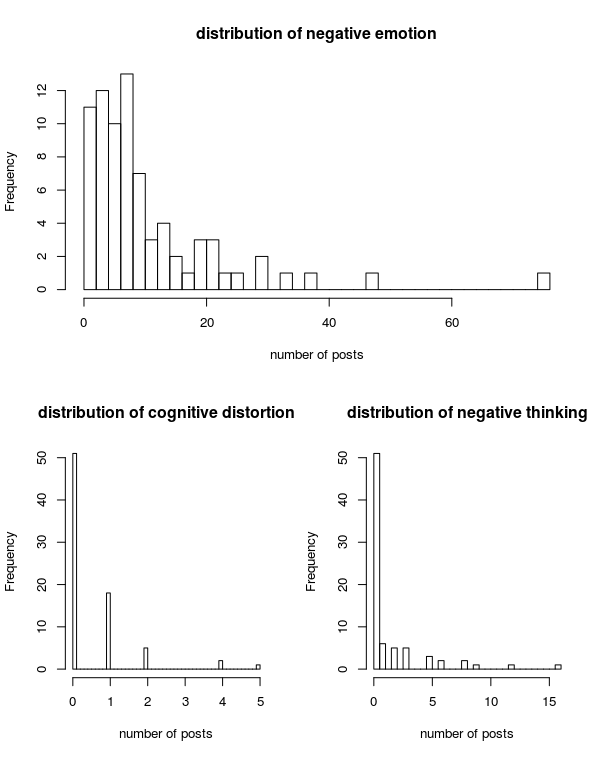
\includegraphics[width=80mm,scale=0.8]{fig1}
  \caption{Distribution of negative emotion and transdiagnostic symptoms}
  \label{fig:one}
\end{figure}

% Head 2
\subsection{Dataset Statistics}

Since cognitive distortion appears to be most correlated with psychopathology Table~\ref{tab:one}, we now subset a sample of individuals with their cognitive distortion score higher than the group mean, which yields a sample of 26 individuals. We also subset another sample in which individuals have lower than average cognitive distortion score (n = 51). We compare depression symptoms, satisfaction with life and personality among the two groups

Figure ~\ref{fig:two} shows the age distribution of the sample population, the high and low cognitive distortion group. The age distribution shows that individuals from 15-20 years old accounted for the majority number of people in our sample population (skewness = 1.685 , kurtosis = 5.532), the same pattern occurs in the low cognitive distortion group  (skewness = 1.332 , kurtosis = 3.911) . Whereas, a majority of the people in the high cognitive distortion group are from 20-22  (skewness = 0.817 , kurtosis = 3.964). 


% Figure
\begin{figure}
  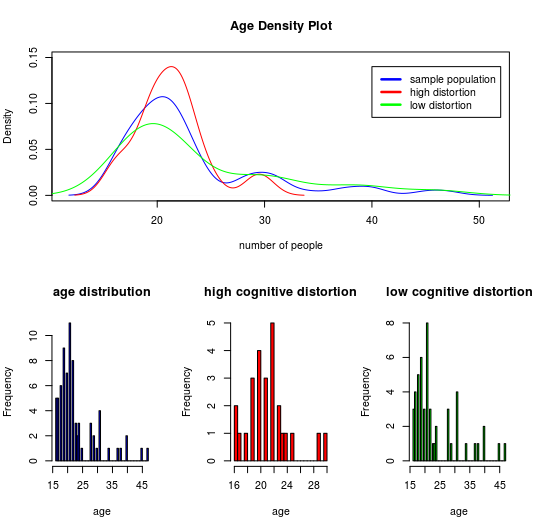
\includegraphics[width=80mm,scale=0.8]{fig2}
  \caption{Distribution of negative emotion and transdiagnostic symptoms}
  \label{fig:two}
\end{figure}


% Figure
\begin{figure}
  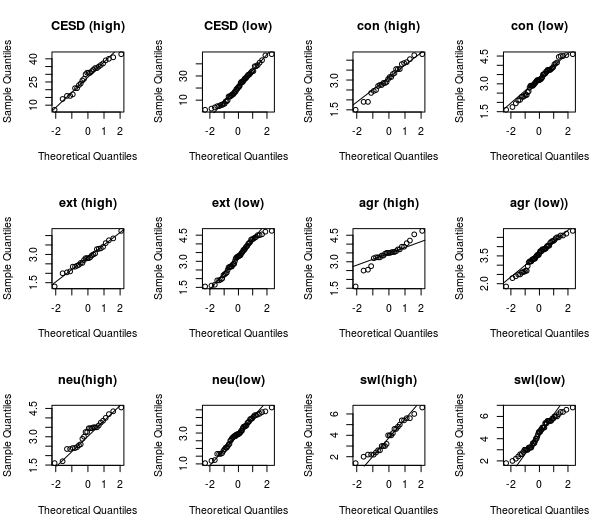
\includegraphics[scale=0.9]{CESD_distortion}
  \caption{qqplot of selected variables}
  \label{fig:three}
\end{figure}


% Table
\begin{table}%
\caption{t-test Between Users with High or Low Transdiagnostic Symptoms}
\label{tab:two}
\begin{minipage}{\columnwidth}
\begin{center}
\begin{tabular}{llllllllll}
  \toprule
        & \multicolumn{2}{c}{all(n=77)}	& \multicolumn{2}{c}{High Trans(n=26)}   & \multicolumn{2}{c}{Low Trans(n=29)} &  &  \\ 
   &  mean  & SD &  mean & SD &  mean & SD & p & Cohen's d \\     

  \hline\hline
  SWL  & 4.221 &  & 3.831 &  &4.483 &  &  & -0.42 \\
  CES-D  & 23.860 &  & 28.42 &  &21.62 &  & * & 0.60 \\
  ope  & 4.166 &  & 4.052 &  &4.148 &  &  &-0.37 \\
  con  & 3.183 &  & 3.085 &  &3.094 &  &  & -0.19\\
  ext  & 3.101 &  & 2.838 &  &3.094 &  &  & -0.48 \\
  agr  & 3.539 &  & 3.457 &  &3.522 &  &  &-0.18 \\
  neu  & 3.022 &  & 3.152 &  &2.96 &  &  & 0.22 \\

\bottomrule
\end{tabular}
\end{center}
\bigskip\centering

 \emph{Note:} * p<0.05, **p<0.01, ***p<0.001 after boferroni correction. Effect size: 0.8 = large(L);  0.5= moderate(M); 0.2 = small(S)
num. of posts: Number of posts in two months;  SWL: Satisfaction with Life score
CES-D: Center for Epidemiological Studies Depression (CESD); ope: openness; con: conscientiousness; ext: extraversion; agr: agreeableness;  neu: neuroticism. 

\end{minipage}
\end{table}%

We present transdiagnostic symptoms scores from the two groups together with their self-reported big-5 personality score, satisfaction with life score and depression symptom score Table ~\ref{tab:two} . Two users didn’t report their age on their profiles, here we assign the mean age to the them. We conduct independent sample t-tests on the selected variables among the two groups. Figure ~\ref{fig:three} shows the qqplot of the selected variables. 

Our observation indicate that users' personality characteristics does not distinguish their transdiagnostic symptoms. However, users with more transdiagnostic symptoms tend to post more posts (nearly twice more than the low symptom group).  They also reported significantly more depression symptoms (28\% higher than low symptom users).

We further divide users according to their demographic characteristics (gender, marital status, relationship status and relationship with parents), and observe their differences in transdiagnostic symptoms Table ~\ref{tab:three}. Users missing some of the characteristics information are assigned under the category 'other', users in this category are not included in this analysis. Since Figure \label{fig:two} shows that the transdiagnostic symptoms and negative emotion are not in normal distribution. We conduct Wilcoxon signed-rank test (non-parametric test used when the sample is not normally distributed) to compare these components between male and female. Result shows that there is no gender difference in transdiagnostic symptoms. 

We attempt to find out if relationship status contribute to the amount of transdiagnostic symptoms. We used Kruskal-Wallis test to compare the median between users with different relationship status: single, be in a relationship, married. Kruskal-Wallis test is a non-parametric equivalent of one-way analysis of variance (ANOVA). ANOVA is used when the residuals are normally distributed, which is not the case in our sample. Whereas, Kruskal-Wallis can be used to compare the median between the groups when this assumption is not satisfied. Result shows the three groups show no statistical significance in negative emotion (H= 4.516, p >0.05), cognitive distortion (H = 1.573, p >0.05) and negative thinking(H = 1.628, p >0.05). Although the median of the three groups appears no difference but the density plots from the three groups show that most of the married individuals have significantly lower transdiagnostic symptom and negative emotion \label{fig:three}. Having a partner to provide mental support seems to be a protective factor, whereas, no difference is found among people being in a relationship. Therefore, the result can be interpreted the other way around, people has a partner and with less transdiagnostic symptoms are more likely to get married or report married on social media. Moreover, individuals without divorced parents tend to have lower negative emotion cognitive distortion and negative thinking compared with those who have divorced parents. 

% Figure
\begin{figure}
  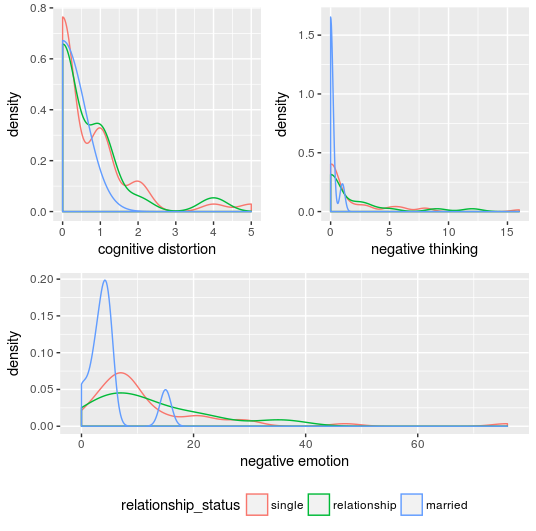
\includegraphics[scale=0.9]{neg_emo_rela}
  \caption{negative emotion in different relationship statuses}
  \label{fig:three}
\end{figure}


% Table
\begin{table}%
\caption{Comparing Transdiagnostic Symptoms Among Different Demographic Groups}
\label{tab:three}
\begin{minipage}{\columnwidth}
\begin{center}
\begin{tabular}{lllllllllll}
  \toprule
        & \multicolumn{2}{c}{parents together}	& \multicolumn{2}{c}{parents NOT together}     \\ 
      & mean &  SD & mean &  SD & p & Hodges-Lehmann estimator \\   
    \hline
    \hline
 Negative emotion  &6.315  & 4.607 & 13.292 &4.607 &* & -0.067 \\
  Cognitive distortion   &0.158  & 0.374 &0.625 &1.095 & &0.000 \\
  Negative thinking  &0.263  & 0.653 & 1.75 &2.937 & &0.000\\
  CES-D  &19.63  & 10.24 & 25.12 &12.74 & & 6.000\\
  \bottomrule
\end{tabular}
\end{center}
\bigskip\centering

 \emph{Note:} * p<0.05, **p<0.01, ***p<0.001. Hodges-Lehmann test estimates the pseudo-median in non-parametric test. Hodges-Lehmann estimator shows the difference between the pseudo-median.

\end{minipage}
\end{table}%


% Head 3
\subsection{Late night posts}
Sleep disturbance is one of the major symptoms in depression. We investigate the relationship between sleep disturbance and cognitive distortion. We count the number of posts written from midnight 12:00am until 6:00am in the morning. Then compute the proportion of late night post to the total number of post of that user. We investigate the relationship between proportion of late night post to transdiagnositic symptoms. For transdiagnositic symptoms, we divide the cumulative symptom by the number of post of the user.

Negative emotion  (r = 0.293, p < 0.01), cognitive distortion (r = 0.300, p < 0.01) and negative thinking (r = 0.285, p <0.05) are slightly correlated with number of late night post. It appears that negative thinking is more likely to occur in late night post. Our result is also supported by the cognitive model of insomnia. Insomnia individuals suffer unpleasant thoughts and excessive, uncontrollable worry during the pre-sleep period (Borkovec 1979, 1982; Morin, 1993). 

% Head 4
\subsection{Linguistics styles}
We also measure the correlation between transdiagnostic components and linguistics style. Linguistics styles capture how an individual use different components of the language in various psychological or social environments. We used LIWC to define the linguistics styles of each Facebook posts, then we aggregate the linguistic style score on user level. Table ~\ref{tab:four} shows the correlation between user linguistics style score and transdiagnostic symptoms. 

Clout refers to the social status, confidence, or leadership that people display through their writing. Study found that people with higher status tend to use less first-person pronoun and use more first-person plural and second-person singular pronoun \cite{Kacewicz13}. It appears in our result that clout is strongly correlated with people with more negative emotions. They tend to focus on self, thus, they use less 3rd person or 2ed person pronouns. Our finding is in correspond to the finding from Pennenaker's depression and language study \cite{Pennebaker10}. The difference of self-focus might be a result in response to emotional pain or a thinking pattern that is a predilection for depression \cite{Wolf07}.

It is not surprised to see that emotional tone, which refers to the positive tone, is negatively correlated with negative emotion score. Negative emotion is also moderately correlated with our manual labeled negative emotion. Social referents, which refers to words indicating social roles (father, mother, sister and so on) are slightly to moderately linked to cognitive distortion and negative emotion. Our result indicates that people shows more negative emotion and cognitive distortion on social media are more likely to be socially detached from family and friends.  We also find that these people are more present and future oriented and use less exclamation marks. However, this might be particular to social media text, because users seldom describe the negative events happen in the past with detail on Facebook posts, instead, they vent out their feelings to the events. For example, 'I am bored.' 'feeling sick again.' 'I hate today.' Exclamation marks is often used to indicate excitement or surprise in a positive context.

It appears that the content of negative thinking is often related to health and home. However, our result is limited to the context of social media, it's likely that people are less open to talk about financial situation and work issues on social media because that could affect their social image. On the other hand, posts that contain cognitive distortion is not content specific, they tend to have longer words and more words in a sentence and these words are more likely to be in the LIWC dictionary. This is mainly due to the fact that there is a lot of reasoning and thinking process in cognitive distortion posts. In addition, the language on cognitive distortion is also less reward focus and more risk or prevention focus.

% Table
\begin{table}%
\caption{Transdiagnositc components and depression symptoms}
\label{tab:four}
\begin{minipage}{\columnwidth}
\begin{center}
\begin{tabular}{llll}
  \toprule
           & Negative emotion & Cognitive distortion  & Negative thinking  \\ 
  \hline\hline
  SUMMARY VARIABLE   \\
  analytic &  & -0.262* &   \\
  clout & -0.518** &   &-0.310**   \\
  authentic &  & 0.325**  &   \\
  emotional tone & -0.341*** &   &   \\
  LANGUAGE MATRICS &  &   &   \\
  words > 6 letters &  & -0.335**  &   \\
  words per sentence &  & 0.258*  &   \\
  dictionary words & 0.234* & 0.412***  &   \\
  GRAMMAR &  &   &   \\
  functional words &  & 0.344**  &   \\
  total pronouns &  & 0.251**  &   \\
  personal pronouns &  & 0.251**  &   \\
  1st per pronoun & 0.369** & 0.325**  & 0.239*  \\
  3rd per singular &-0.326*& -0.249* &    \\
  2nd person & -0.235* &   &   \\
  prepositions &  & 0.273*  &   \\
  conjunctions &0.322**  & 0.309*  &   \\
  adjective &  & 0.270*  &   \\
  comparatives &  & 0.320**  &   \\
  verb & 0.244* &   &   \\
  AFFECT WORDS &  &   &   \\
  negative emotion &0.322**  &   &   \\
  anger &0.413***  &   &   \\
  anxiety &  &   &   \\
  sadness &  &   &   \\
  swear & 0.385*** &   &   \\
  SOCIAL  &  &   &   \\
  social words &  &   & -0.263*  \\
  female referents &-0.338** & -0.237* &     \\
  male referents &  & -0.261*  &   \\
  COGNITIVE PROCESS &  &   &   \\
  differentiation &0.323**  &   &   \\
  PERCEPTUAL &  &   &   \\
  perceptual process &  &0.255*   &   \\
  feeling &  & 0.301*  &   \\
  BIOLOGICAL &  &   &   \\
  health/illness &  &   & 0.335*  \\
  CORE DRIVE &  &   &   \\
  reward focus &  & -0.249*  &   \\
  risk/prevention focus &  & 0.312**  &   \\
  TIME &  &   &   \\
  present focus & 0.247* & 0.232*  &   \\
  future focus &0.312*  &   &   \\
  PERSONAL CONCERN &  &   &   \\
  home & 0.300** &   &   0.246*\\
  work &  &   &   \\
  money &  &   &   \\
  PUNCTUATION &  &   &   \\
  exclamation marks &-0.257*  &-0.317*   &   \\
  


  \bottomrule
\end{tabular}
\end{center}
\bigskip\centering

 \emph{Note:} * p<0.05, **p<0.01, ***p<0.001 

\end{minipage}
\end{table}%

% Head 4
\subsection{Cognitive Distortion Regression Model}

We explore the performance of a linear regression model in predicting cognitive distortion. We found high interactions between the LIWC features. Whereas, PCA or SVD-based feature selection methods do not take into account the potential multivariate nature of the data structure. We select features that are most correlated with cognitive distortion according to Table~\ref{tab:four}. "Dictionary words" has the highest correlation with cognitive distortion but also has high interaction with more 1/3 of the language features, therefore, we removed "dictionary words" to avoid multivariation. Then we further remove features that are more than 0.3 correlated with the top features. Our model explains 52\% of variance in the data. Swear words and Risk focus are very strong predictors.

% Table
\begin{table}%
\caption{Cognitive Distortion Linear Regression Model}
\label{tab:five}
\begin{minipage}{\columnwidth}
\begin{center}
\begin{tabular}{lllll}
  \toprule
        measures & beta	& SE   & t-Stat \\
  \hline
  \hline 
Intercept        &   0.199  &0.160 &  1.240  \\ 
total pronouns&  0.010* &  0.004 &  2.221 \\
3rd person pronoun  & -0.019*  & 0.008 & -2.291   \\
preposition   &  0.021**  & 0.007 &  2.837  \\
swear  &  0.021***  & 0.005 &  4.026\\
feeling   &  0.029**  & 0.010 &  2.929  \\
reward focus & -0.020*  & 0.009 & -2.132 \\
risk focus   &  0.030***  & 0.008 &  3.494 \\
proportion of late night post        &   1.031*  & 0.426 &  2.417 \\

  \hline
  Residual standard error &  0.714  \\
  Multiple-R2 &  0.521 \\ 
  Error degrees of freedom  & 68  \\ 
  \hline
  \bottomrule
\end{tabular}
\end{center}
\bigskip\centering

 \emph{Note:} . < 0.1 * p<0.05, **p<0.01, ***p<0.001 
parents not together1: no and not in contact with mother; parents not together2: no but in frequent contact with parents; 

\end{minipage}
\end{table}%

\section{CONCLUSION}
This research is designed as an approach to complement the current transdiagnositic diagnostic approach with a novel way to access people's behavior. We examine the feasibility to identify transdiagnostic symptoms using Facebook data and finding out the language features that are able to predict cognitive distortion, a core component in CBT, which is highly associated with anxiety and depressive disorders. First, we label negative emotion, cognitive distortion and negative thinking in more than 4000 Facebook posts. Then we investigate the relationship between these components and depression symptoms, satisfaction with life and big-5 personality. Thereafter, we characterize the differences of transdiagnostic symptoms and negative emotions among different demographic groups. Finally, we identify features that are able to predict cognitive distortion.

We found that cognitive distortion is moderately correlated with depression symptoms and satisfaction with life. Marriage and without divorced parents seem to be protective factors in developing transdiagnostic symptoms. We found that some of the language features are best predicting cognitive distortion (explained 55\% of variance in the data). The proportion of posts written at mid night, which is a sign of insomnia, also enhance the prediction. 

The major limitation of our work is that our data is from social media platform. Facebook data may not represent the thinking process of an individual most precisely, because users have different degree of selective biased presentation and self-disclosure level. Moreover, this work focus on a limited set of sample that involve 77 users. It would be useful to replicate the study on a larger population to validate the pattern we found in here. 





%\chapter{Research plan and progress}  
\section{First Year}
The first two months of the academic year were spent on reviewing the literature relevant to my research field, identifying the research gap and planning for my first study about identifying cognitive distortion on social media posts. The next six months were spent on drafting the annotation guideline, manually annotating the sample by myself and conducting the analysis. By the 8th month, the a conference paper based on the analysis was completed, but we decide to recruit students to relabel the task in order to validate my annotation. The next five months were spent on my second study about social support on reddit. I designed the study and collected data on the 9th month. From 10th - 12 months, I analysis the data and drafted a conference paper based on some of the findings. We submitted my second study to CHI 2019 at the 12th month. Then I spent the 13th month to prepare for the proposal presented in here and meanwhile working on my first study. 

\section{Second Year}
We are developing an annotation tool for the annotation of the cognitive distortion project. The annotation is expected to be completed on the 14th month, then I will redo the analysis and modify the draft of the paper. The cognitive distortion project focuses on monitoring valence (indicative of stress) and its interaction with vulnerability factors such as personality, satisfaction with life and self-disclosure level. The interaction between stress and vulnerability is an important underlying mechanism for the development of psychological disorders. Another objective of this study is to inspect whether cognitive distortion as a perpetuating mental health risk can be identified on social media. The cognitive distortion project is expected to be completed by the 15th month.

After that, we will extract the questions asked by the post author the social support study and cluster the questions according to their language attributes. The we will submit a short paper based on this analysis to another conference at the 16th month. On the 17th month, I am planning to expand the data from the previous reddit study by collect and analyzing posts from the same set of participants in other reddit communities. The aim of this study is to inspect whether people show more greater distress when disclosing a stressful life events endorse certain types of reddit communities and what are their language characteristics in various topics. We will analyze the topics, valence, language attributes and cognitive flexibility from the posts. This work is expected to be completed by 22th month. 

Then we will move on to the third project about chronic stress. Stressful events detection has been widely studied using social media data, whereas, chronic stress remains a research gap in this field. In the first stage, we intend to observe the characteristics from people who disclose a specific type of role stress on social media, such as being a care taker of children with autism. Then we compare their disclosure of chronic stress with those who suffer from a sudden stressful life events. The social support needs and support provided by the audiences will be characterized.

\section{Third Year}
In the second stage of the chronic stress project, we also inspect how people with strong or weak social ties disclose chronic stress on non-anonymous social media. Strong social ties have a buffering effect on stressful life experience. If strong ties are not available, people often seek support from the weak ties. We intend to compare the support provided by weak ties with those from strong ties. We will also observe the poster's interaction with the audiences. By inspecting how people with more strong ties maintain and develop social ties, we intend to provide insight for future design that help people to strengthen their social ties. The chronic stress study is expected to be finished on 26th months. 

The 27th - 31 months will be spent on cross-cultural studies. We will observe if there's any cultural differences in some of our previous findings. we intend to replicate some of the previous studies on a set of data from a Chinese forum called 'Tianya'. Then I will dedicate the rest of my PhD time on the dissertation \ref{fig:one}. 

% Figure
\begin{figure}
  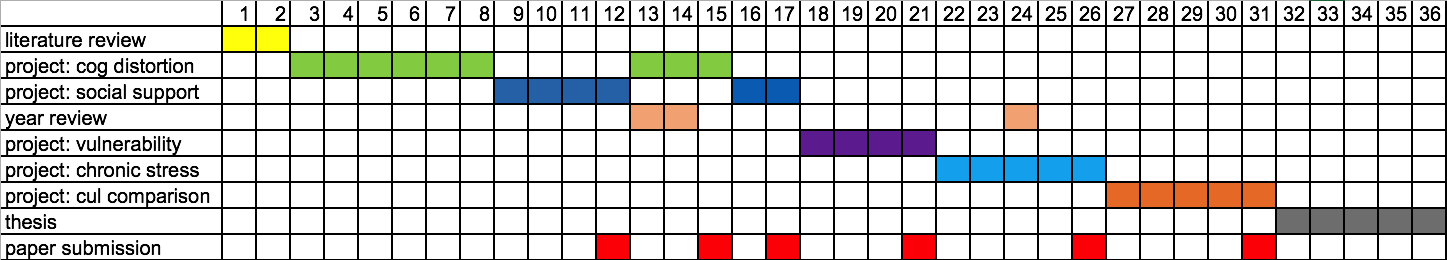
\includegraphics[width=160mm,scale=1.5]{Chapter5/timeline.png}
  \caption{PhD Timeline}
  \label{fig:one}
\end{figure}

%\include{Chapter6/chapter6}
%\include{Chapter7/chapter7}



% ********************************** Back Matter *******************************
% Backmatter should be commented out, if you are using appendices after References
%\backmatter

% ********************************** Bibliography ******************************
\begin{spacing}{0.9}

% To use the conventional natbib style referencing
% Bibliography style previews: http://nodonn.tipido.net/bibstyle.php
% Reference styles: http://sites.stat.psu.edu/~surajit/present/bib.htm

%\bibliographystyle{apalike}
%\bibliographystyle{unsrt} % Use for unsorted references  
\bibliographystyle{plainnat} % use this to have URLs listed in References
\cleardoublepage
\bibliography{References/myref} % Path to your References.bib file


% If you would like to use BibLaTeX for your references, pass `custombib' as
% an option in the document class. The location of 'reference.bib' should be
% specified in the preamble.tex file in the custombib section.
% Comment out the lines related to natbib above and uncomment the following line.

%\printbibliography[heading=bibintoc, title={References}]


\end{spacing}

% ********************************** Appendices ********************************

\begin{appendices} % Using appendices environment for more functunality

%!TEX root = ../thesis.tex
% ******************************* Thesis Appendix A ****************************
\chapter{How to install \LaTeX} 

\section*{Windows OS}

\subsection*{TeXLive package - full version}
\begin{enumerate}
\item	Download the TeXLive ISO (2.2GB) from\\
\href{https://www.tug.org/texlive/}{https://www.tug.org/texlive/}
\item	Download WinCDEmu (if you don't have a virtual drive) from \\
\href{http://wincdemu.sysprogs.org/download/}
{http://wincdemu.sysprogs.org/download/}
\item	To install Windows CD Emulator follow the instructions at\\
\href{http://wincdemu.sysprogs.org/tutorials/install/}
{http://wincdemu.sysprogs.org/tutorials/install/}
\item	Right click the iso and mount it using the WinCDEmu as shown in \\
\href{http://wincdemu.sysprogs.org/tutorials/mount/}{
http://wincdemu.sysprogs.org/tutorials/mount/}
\item	Open your virtual drive and run setup.pl
\end{enumerate}

or

\subsection*{Basic MikTeX - \TeX~ distribution}
\begin{enumerate}
\item	Download Basic-MiK\TeX (32bit or 64bit) from\\
\href{http://miktex.org/download}{http://miktex.org/download}
\item	Run the installer 
\item	To add a new package go to Start >> All Programs >> MikTex >> Maintenance (Admin) and choose Package Manager
\item	Select or search for packages to install
\end{enumerate}

\subsection*{TexStudio - \TeX~ editor}
\begin{enumerate}
\item	Download TexStudio from\\
\href{http://texstudio.sourceforge.net/\#downloads}
{http://texstudio.sourceforge.net/\#downloads} 
\item	Run the installer
\end{enumerate}

\section*{Mac OS X}
\subsection*{MacTeX - \TeX~ distribution}
\begin{enumerate}
\item	Download the file from\\
\href{https://www.tug.org/mactex/}{https://www.tug.org/mactex/}
\item	Extract and double click to run the installer. It does the entire configuration, sit back and relax.
\end{enumerate}

\subsection*{TexStudio - \TeX~ editor}
\begin{enumerate}
\item	Download TexStudio from\\
\href{http://texstudio.sourceforge.net/\#downloads}
{http://texstudio.sourceforge.net/\#downloads} 
\item	Extract and Start
\end{enumerate}


\section*{Unix/Linux}
\subsection*{TeXLive - \TeX~ distribution}
\subsubsection*{Getting the distribution:}
\begin{enumerate}
\item	TexLive can be downloaded from\\
\href{http://www.tug.org/texlive/acquire-netinstall.html}
{http://www.tug.org/texlive/acquire-netinstall.html}.
\item	TexLive is provided by most operating system you can use (rpm,apt-get or yum) to get TexLive distributions
\end{enumerate}

\subsubsection*{Installation}
\begin{enumerate}
\item	Mount the ISO file in the mnt directory
\begin{verbatim}
mount -t iso9660 -o ro,loop,noauto /your/texlive####.iso /mnt
\end{verbatim}

\item	Install wget on your OS (use rpm, apt-get or yum install)
\item	Run the installer script install-tl.
\begin{verbatim}
	cd /your/download/directory
	./install-tl
\end{verbatim}
\item	Enter command `i' for installation

\item	Post-Installation configuration:\\
\href{http://www.tug.org/texlive/doc/texlive-en/texlive-en.html\#x1-320003.4.1}
{http://www.tug.org/texlive/doc/texlive-en/texlive-en.html\#x1-320003.4.1} 
\item	Set the path for the directory of TexLive binaries in your .bashrc file
\end{enumerate}

\subsubsection*{For 32bit OS}
For Bourne-compatible shells such as bash, and using Intel x86 GNU/Linux and a default directory setup as an example, the file to edit might be \begin{verbatim}
edit $~/.bashrc file and add following lines
PATH=/usr/local/texlive/2011/bin/i386-linux:$PATH; 
export PATH 
MANPATH=/usr/local/texlive/2011/texmf/doc/man:$MANPATH;
export MANPATH 
INFOPATH=/usr/local/texlive/2011/texmf/doc/info:$INFOPATH;
export INFOPATH
\end{verbatim}
\subsubsection*{For 64bit OS}
\begin{verbatim}
edit $~/.bashrc file and add following lines
PATH=/usr/local/texlive/2011/bin/x86_64-linux:$PATH;
export PATH 
MANPATH=/usr/local/texlive/2011/texmf/doc/man:$MANPATH;
export MANPATH 
INFOPATH=/usr/local/texlive/2011/texmf/doc/info:$INFOPATH;
export INFOPATH

\end{verbatim}



%\subsection{Installing directly using Linux packages} 
\subsubsection*{Fedora/RedHat/CentOS:}
\begin{verbatim} 
sudo yum install texlive 
sudo yum install psutils 
\end{verbatim}


\subsubsection*{SUSE:}
\begin{verbatim}
sudo zypper install texlive
\end{verbatim}


\subsubsection*{Debian/Ubuntu:}
\begin{verbatim} 
sudo apt-get install texlive texlive-latex-extra 
sudo apt-get install psutils
\end{verbatim}

%!TEX root = ../thesis.tex
% ******************************* Thesis Appendix B ********************************

\chapter{Installing the CUED class file}

\LaTeX.cls files can be accessed system-wide when they are placed in the
<texmf>/tex/latex directory, where <texmf> is the root directory of the user’s \TeX installation. On systems that have a local texmf tree (<texmflocal>), which
may be named ``texmf-local'' or ``localtexmf'', it may be advisable to install packages in <texmflocal>, rather than <texmf> as the contents of the former, unlike that of the latter, are preserved after the \LaTeX system is reinstalled and/or upgraded.

It is recommended that the user create a subdirectory <texmf>/tex/latex/CUED for all CUED related \LaTeX class and package files. On some \LaTeX systems, the directory look-up tables will need to be refreshed after making additions or deletions to the system files. For \TeX Live systems this is accomplished via executing ``texhash'' as root. MIK\TeX users can run ``initexmf -u'' to accomplish the same thing.

Users not willing or able to install the files system-wide can install them in their personal directories, but will then have to provide the path (full or relative) in addition to the filename when referring to them in \LaTeX.

\end{appendices}

% *************************************** Index ********************************
\printthesisindex % If index is present

\end{document}
